%%%%%%%%%%%%%%%%%%%%%%%%%%%%%%%%%%%%%%%%%
% Jacobs Landscape Poster
% LaTeX Template
% Version 1.1 (14/06/14)
%
% Created by:
% Computational Physics and Biophysics Group, Jacobs University
% https://teamwork.jacobs-university.de:8443/confluence/display/CoPandBiG/LaTeX+Poster
% 
% Further modified by:
% Nathaniel Johnston (nathaniel@njohnston.ca)
%
% This template has been downloaded from:
% http://www.LaTeXTemplates.com
%
% License:
% CC BY-NC-SA 3.0 (http://creativecommons.org/licenses/by-nc-sa/3.0/)
%
%%%%%%%%%%%%%%%%%%%%%%%%%%%%%%%%%%%%%%%%%

%----------------------------------------------------------------------------------------
%	PACKAGES AND OTHER DOCUMENT CONFIGURATIONS
%----------------------------------------------------------------------------------------

\documentclass[final]{beamer}

\usepackage[scale=1.24]{beamerposter} % Use the beamerposter package for laying out the poster

\usetheme{confposter} % Use the confposter theme supplied with this template

\setbeamercolor{block title}{fg=ngreen,bg=white} % Colors of the block titles
\setbeamercolor{block body}{fg=black,bg=white} % Colors of the body of blocks
\setbeamercolor{block alerted title}{fg=white,bg=dblue!70} % Colors of the highlighted block titles
\setbeamercolor{block alerted body}{fg=black,bg=dblue!10} % Colors of the body of highlighted blocks
% Many more colors are available for use in beamerthemeconfposter.sty

%-----------------------------------------------------------
% Define the column widths and overall poster size
% To set effective sepwid, onecolwid and twocolwid values, first choose how many columns you want and how much separation you want between columns
% In this template, the separation width chosen is 0.024 of the paper width and a 4-column layout
% onecolwid should therefore be (1-(# of columns+1)*sepwid)/# of columns e.g. (1-(4+1)*0.024)/4 = 0.22
% Set twocolwid to be (2*onecolwid)+sepwid = 0.464
% Set threecolwid to be (3*onecolwid)+2*sepwid = 0.708

\newlength{\sepwid}
\newlength{\onecolwid}
\newlength{\twocolwid}
\newlength{\threecolwid}
\setlength{\paperwidth}{48in} % A0 width: 46.8in
\setlength{\paperheight}{36in} % A0 height: 33.1in
\setlength{\sepwid}{0.024\paperwidth} % Separation width (white space) between columns
\setlength{\onecolwid}{0.22\paperwidth} % Width of one column
\setlength{\twocolwid}{0.464\paperwidth} % Width of two columns
\setlength{\threecolwid}{0.708\paperwidth} % Width of three columns
\setlength{\topmargin}{-0.5in} % Reduce the top margin size
%-----------------------------------------------------------

\usepackage{graphicx}  % Required for including images

\usepackage{booktabs} % Top and bottom rules for tables

%----------------------------------------------------------------------------------------
%	TITLE SECTION 
%----------------------------------------------------------------------------------------

\title{Classification for the Yelp Data Set Challenge} % Poster title

\author{Nicolas Drizard \& Virgile Audi} % Author(s)

\institute{CS281 Final Project, Harvard University} % Institution(s)

%----------------------------------------------------------------------------------------

\begin{document}

\addtobeamertemplate{block end}{}{\vspace*{2ex}} % White space under blocks
\addtobeamertemplate{block alerted end}{}{\vspace*{2ex}} % White space under highlighted (alert) blocks

\setlength{\belowcaptionskip}{2ex} % White space under figures
\setlength\belowdisplayshortskip{2ex} % White space under equations

\begin{frame}[t] % The whole poster is enclosed in one beamer frame

\begin{columns}[t] % The whole poster consists of three major columns, the second of which is split into two columns twice - the [t] option aligns each column's content to the top

\begin{column}{\sepwid}\end{column} % Empty spacer column

\begin{column}{\onecolwid}\vspace{-0.6in} % The first column

%----------------------------------------------------------------------------------------
%	OBJECTIVES
%----------------------------------------------------------------------------------------

\begin{alertblock}{Objectives}
\small
We are taking part in the Yelp Dataset challenge round 6. We chosed to solve the question of infering categories based on the reviews. The goal is to build a finer way to categorize the Yelp businesses.\\

Our approach consists in using Latent Dirichlet Allocation to build latent features from the text reviews which would depict the categories of each business and turn it into a vector representation which carries local geometry information. We then resorted to building a network of restaurant based on this underlying geometry and cluster this network using a graph theory algorithm.\\

\end{alertblock}

%----------------------------------------------------------------------------------------
%	INTRODUCTION
%----------------------------------------------------------------------------------------

\begin{block}{The Data}
\small
\begin{itemize}
		\item 1.6 million reviews
		\item 61 000 businesses
		\item 481 000 attributes (ie hours, parking availabity, take-out, ambience)
		\item aggregated check-in measurements over time
\end{itemize}

We cleaned and prepared restaurants data in the city of Las Vegas, NV to grasp in a finer manner the local relationships of the restaurants. This also makes more sense on from the user's perspective.\\

\end{block}

\begin{block}{Latent Dirichlet Allocation}
\small

LDA \cite{LDA} is a three-level hierarchical Bayesian model. Documents are represented as random mixtures over latent topics and each topic is characterized by a distribution over words. \\
The generative process for a document \textbf{w} in a corpus D is the following:
\begin{enumerate}
	\item Choose the topics representation $\phi \sim$ Dir($\beta$)
	\item Choose the number of words: $ N \sim $ Poisson($ \xi $)
	\item Choose the distribution of topics $\theta_w \sim$ Dir($\alpha_w$)
	\item For each of the N words:
	\begin{enumerate}
		\item Choose a topic assignement $z_{n,w} \sim$ Multinomial($\theta_w$)
		\item Choose a word $w_n \sim$ Multinomial($\phi_{z_{n,w}}$)
	\end{enumerate}
\end{enumerate}
We chose an online variational inference algorithm \cite{OLLD} which showed significant speed improvement when compared to the LDA python package using Gibbs sampling. To fit an LDA model with 50 topics on a 4000 document corpus and 10000 words took:
$$ \text{Online} = 1m13s \quad \text{Gibbs} = 50m $$
\end{block}
%------------------------------------------------

\begin{figure}
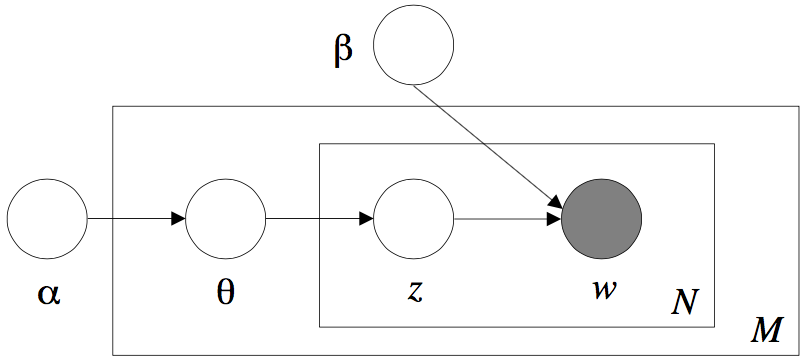
\includegraphics[width=0.5\linewidth]{LDA.png}
\caption{Graphical Model Representation of LDA}
\end{figure}

%----------------------------------------------------------------------------------------

\end{column} % End of the first column

\begin{column}{\sepwid}\end{column} % Empty spacer column

\begin{column}{\twocolwid} % Begin a column which is two columns wide (column 2)
\begin{figure}
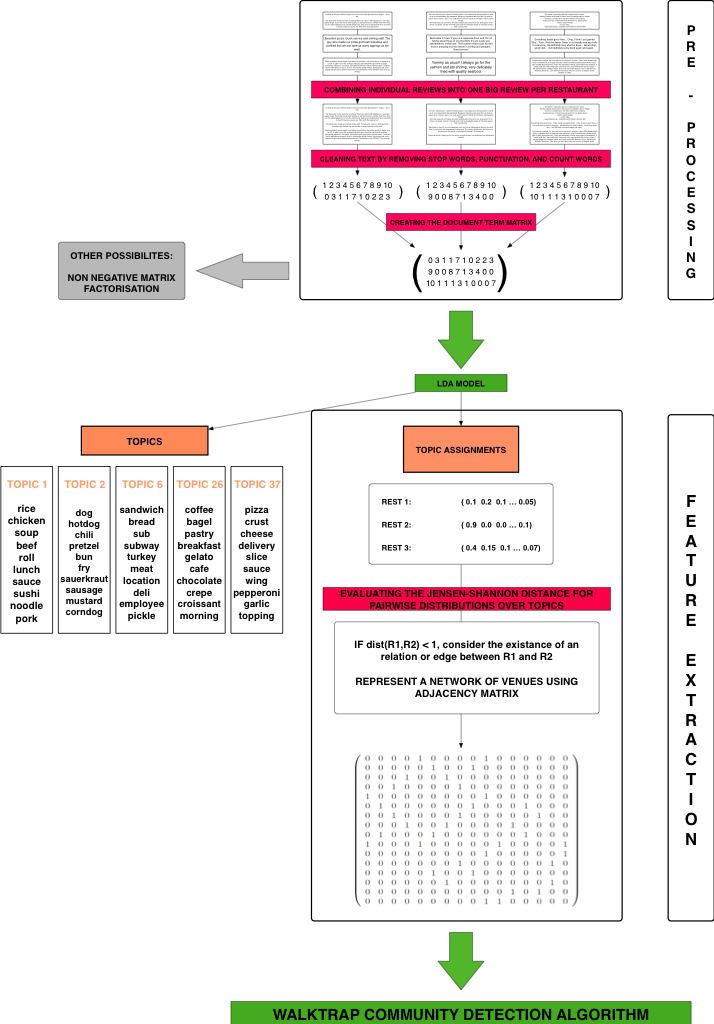
\includegraphics[width=0.6\linewidth]{posterpicture3.jpg}
\end{figure}

\begin{column}{\twocolwid} % The first column within column 2 (column 2.1)
\begin{figure}

\includegraphics[width=1\linewidth]{dendo_3-1.png}
\caption{Overall Process}
\end{figure}

\end{column}

\begin{columns}[t,totalwidth=\twocolwid]\hspace{-0.6in} % Split up the two columns wide column again

\begin{column}{\onecolwid} % The first column within column 2 (column 2.1)

%----------------------------------------------------------------------------------------
%	MATHEMATICAL SECTION
%----------------------------------------------------------------------------------------

\begin{block}{Evaluation}
\small
Perplexity is defined as the geometric mean of the log likelihood of the words in the held-out set of docuements given the trained model. In our case, for each document we held out 20\% of the words which constitue the test set.
\end{block}

%----------------------------------------------------------------------------------------

\end{column} % End of column 2.1

\begin{column}{\onecolwid}\hspace{-0.6in} % The second column within column 2 (column 2.2)

%----------------------------------------------------------------------------------------
%	RESULTS
%----------------------------------------------------------------------------------------
\small
\vfill{The formula is given by:}
\begin{center}
$$
	\boxed{\quad\text{perp}(D_{test}) = \frac{\sum_{d \in D_{test}} \sum_{w \in d} \log \left( \sum_{t \in topics} p(w|t) p(t|d) \right)}{\sum_{d \in D_{test}|d|}}\quad}
$$

\end{center}
%----------------------------------------------------------------------------------------

\end{column} % End of column 2.2

\end{columns} % End of the split of column 2

%----------------------------------------------------------------------------------------


\end{column} % End of the second column

\begin{column}{\sepwid}\end{column} % Empty spacer column

\begin{column}{\onecolwid}\vspace{-0.6in} % The third column

%----------------------------------------------------------------------------------------
%	CONCLUSION
%-----------------------------------------------------------
\begin{block}{Graph Theory}
\small
 The intuition behind the Walktrap algorithm is that random walks on a graph tend to get "trapped into densely connected parts corresponding to communities".\cite{Gr} It is a clustering algorithm based on the definition of a new metric to evaluate the distance between two vertices in a graph:
 $$r_{ij} = \sqrt{\sum\limits_{k=1}^{n}\frac{(P^t_{ik}-P^t_{kj})^2}{d(k)}}$$
 where $P^t_{ik}$ is the transition probability at time t and $d(k)$ is the degree of node k (number of edges incident to the vertex)
\end{block}

%----------------------------------------------------------------------------------------
%	ADDITIONAL INFORMATION
%----------------------------------------------------------------------------------------

\begin{block}{Results}\vspace{-0.2in}
\small
\begin{itemize}
\item The validation indicate that \textbf{50} was the optimum number of topics, some of these topics are plotted in the diagram 
\item Based on the Shannon distance (symmetric KL divergence) between two documents, we set a threshold of 1 and created the adjacency matrix
\item In order to inspect the graph and due to its extremely large size ($\>2 10^{6}$ edges), we sampled 500 restaurants having among their tags either "Chinese", "Seafood" or "Mexican"
\item We ran the walktrap clustering algorithm in R. It initialy found 7 cliques, but a closer insepction of the dendogram, we actually noticed that it subcategories 3 bigger cliques boxed in green, red, and blue, which corresponded almost exactly to the 3 classes of restaurants !
\end{itemize}


\end{block}
\begin{alertblock}{Conclusion}
\small
By using a combination of unsupervised learning and graph theory, we managed to retrieve most of the original classification that is up to now still done at hand ! This work could result in an au tomation tool for Yelp to label properly its data based. 
\end{alertblock}

\begin{block}{Next steps}\vspace{-0.2in}
\small
Futur work could focus on the sub-cliques and try to get a more refine classification by combining them with other features like check-ins, parking availability, etc. As a variant, we could also try a supervised LDA, where we use the existing categories as a response variable associated with each document and infer the joint model of the documents and the responses.
\end{block}

%----------------------------------------------------------------------------------------
%	REFERENCES
%----------------------------------------------------------------------------------------

\begin{block}{References}
\nocite{*} % Insert publications even if they are not cited in the poster
\tiny{\bibliographystyle{unsrt}
\bibliography{sample}}

\end{block}


\end{column} % End of the third column

\end{columns} % End of all the columns in the poster

\end{frame} % End of the enclosing frame

\end{document}
